\documentclass[12pt]{article}

%\usepackage[cm]{fullpage}
\setlength{\topmargin}{-1in}
\setlength{\oddsidemargin}{-0.25in}
\setlength{\evensidemargin}{-0.25in}
\setlength{\textwidth}{7in}
\setlength{\textheight}{9in}


\usepackage{tikz}
\usetikzlibrary{backgrounds}
\usetikzlibrary{arrows,arrows.meta,matrix}
\usetikzlibrary{decorations}
\usetikzlibrary{animations}
\usetikzlibrary{tikzmark,calc}
\usetikzlibrary{bending, positioning}
\usetikzlibrary{3d}
% do not indent outermost itemize environ
%\setlength{\leftmargini}{0in}
%
%\usepackage{hyperref}
\usepackage{multicol}
\usepackage{graphicx}
\usepackage{amsmath}
\usepackage{amssymb}
\usepackage{mathrsfs}
\newcommand{\ds}{\displaystyle}
\renewcommand{\Re}{\mbox{Re}}
\renewcommand{\Im}{\mbox{Im}}
\newcommand{\Arg}{\mbox{Arg}}
\newcommand{\Ln}{\mbox{Ln}}
\renewcommand{\L}{\mathscr{L}}
%\renewcommand{\arraystretch}{1.5}
\usepackage{enumitem}
\usepackage{hyperref}
\usepackage{amssymb}
\usepackage{amsmath}
\usepackage{multicol}
\usepackage{array, latexsym}
\usepackage{times}
\usepackage{time}
\usepackage{subfigure}
\usepackage{graphics}
\usepackage{graphicx}
\usepackage{epstopdf}
\usepackage[T1]{fontenc}
\usepackage{setspace}
\newcommand{\To}{\Rightarrow}
\newcommand{\del}{\nabla}
\newcommand{\R}{\mathbb{R}}
\newcommand{\C}{\mathcal{C}}
\newcommand{\N}{\mathcal{N}}
\newcommand{\A}{\mathcal{A}}
\renewcommand{\O}{\mathcal{O}}
% \renewcommand{\N}{\mathbb{N}}
\newcommand{\ben}{\begin{enumerate}}
\newcommand{\een}{\end{enumerate}}
\newcommand{\eps}{\varepsilon}
\renewcommand{\epsilon}{\varepsilon}
\newcommand{\p}{\partial}
\newcommand{\<}{\langle}
\renewcommand{\>}{\rangle}
\renewcommand{\subset}{\subseteq}
\newcommand{\cont}{\Rightarrow \Leftarrow}
\newcommand{\back}{\backslash}
\newcommand{\norm}[1]{\|{#1}\|}
\newcommand{\abs}[1]{|{#1}|}
\newcommand{\ip}[1]{\langle{#1}\rangle}
\newcommand{\m}[1]{{\mathbf{#1}}}
\newcommand{\sts}{\m{S}^\textrm{T}\m{S}}
\newcommand{\rank}{\textrm{rank}}
\newcommand{\X}{\mathcal{X}}
\newcommand{\Y}{\mathcal{Y}}
\renewcommand{\L}{\mathscr{L}}
\def\ds{\displaystyle}
\def\d{\partial}

\def\plottingAxesSmall{
	\begin{tikzpicture}[samples=100, scale=0.9]

		% === figure/domain/tick bounds ===
		\def\tmin{-3.0}	\def\tmax{5.1}
		\def\ymin{-2.0}	\def\ymax{3.1}
		\def\tticks{-2, -1, 1, 2, 3, 4}
		\def\yticks{-1, 1, 2}

		% === Axes ===
		\draw[->] (\tmin	,0		) -- (\tmax	,0		);
		\draw[->] (0		,\ymin	) -- (0		,\ymax	);
		% \node[font=\small, below] at (\tmax - 0.1	, 0) {$t$};

		% === Tick marks/numeric labels ===
		\foreach \t in \tticks {
			\draw[gray]	(\t,0.1) -- (\t,-0.1);					% t ticks
			\node[below, font=\small] at (\t,-0.08) {\t};	% t labels
			
		}
		\foreach \y in \yticks {
			\draw[gray]	(0.1,\y) -- (-0.1,\y);				% y ticks
			\node[right, font=\small] at (0,\y) {\y};	% y labels
		}
		\draw[very thin,color=lightgray] (\tmin,\ymin) grid (\tmax,\ymax);	
	\end{tikzpicture}
}
\def\plottingAxesBig{
	\begin{tikzpicture}[samples=100, scale=1.0]

		% === figure/domain/tick bounds ===
		\def\tmin{-2.0}	\def\tmax{10.1}
		\def\ymin{-5.0}	\def\ymax{5.1}
		\def\tticks{-2, -1, 1, 2, 3, 4, 5, 6, 7, 8, 9, 10}
		\def\yticks{-4, -3, -2, -1, 1, 2, 3, 4, 5}

		% === Axes ===
		\draw[->] (\tmin	,0		) -- (\tmax	,0		);
		\draw[->] (0		,\ymin	) -- (0		,\ymax	);
		% \node[font=\small, below] at (\tmax - 0.1	, 0) {$t$};

		% === Tick marks/numeric labels ===
		\foreach \t in \tticks {
			\draw[gray]	(\t,0.1) -- (\t,-0.1);					% t ticks
			\node[below, font=\small] at (\t,-0.08) {\t};	% t labels
			
		}
		\foreach \y in \yticks {
			\draw[gray]	(0.1,\y) -- (-0.1,\y);				% y ticks
			\node[right, font=\small] at (0,\y) {\y};	% y labels
		}
		\draw[very thin,color=lightgray] (\tmin,\ymin) grid (\tmax,\ymax);
	\end{tikzpicture}
}

\pagestyle{empty}
\begin{document}

	\noindent\rule{7in}{0.4pt}

	\medskip

	{\centering {\sc Differential Equations - Unit Step Functions}}

	\noindent\rule{7in}{0.4pt}
	
	\medskip

	\noindent {\bf Definition:} The {\it unit step function} $u(t)$ is defined as:
		\[ u(t) = \left\{
		\begin{array}{ll}
			0,	& t<0\\
			1,	&t \ge 0\\
		\end{array} \right.
		\]
	
	\ben
		\item $u(2) = $
		\vspace{0.05cm}
		\item $u(5.32) = $
		\vspace{0.05cm}
		\item $u(-1.2) = $
		\vspace{0.05cm}
		% \item  What is the value of $u(k),$ where $k$ is a positive constant?
		% \vfill
		% \item  What is the value of $u(k),$ where $k$ is a negative constant?
		% \vfill
		\item  Sketch $u(t).$
		
		\centering\plottingAxesSmall

	\een

	\noindent The horizontally {\it shifted unit step function} $u_c(t)$ is given by:
	\[ u_c(t) = u(t-c) = \left\{
	\begin{array}{ll}
		0,	& t<c\\
		1,	&t \ge c\\
	\end{array} \right.
	\]

	\noindent Consider the function $u_3(t).$

	\ben[resume]

		\item $u_3(2) = $
		\vspace{0.05cm}
		\item $u_3(7.43) = $
		\vspace{0.05cm}
		\item $u_3(-1) = $
		\vspace{0.05cm}
		% \item  What is the value of $u_3(k),$ where $k>3$
		% \vfill
		% \item  What is the value of $u_3(k),$ where $k<3$?
		% \vfill
		\item  Sketch $u_3(t).$
			
		\centering\plottingAxesSmall
	\een
	
	\newpage

	\noindent For each of the following, write the function as a piecewise defined function and sketch the function.
	\ben[resume]
    
		\item  Sketch $u_1(t).$
		
		\mbox{}\hfill\plottingAxesSmall
    	\vfill
		
		\item  Sketch $-2u_2(t).$
		
    	\mbox{}\hfill\plottingAxesSmall
    	\vfill
    
		\item  Sketch $3 - 3u_2(t).$
		
    	\mbox{}\hfill\plottingAxesSmall
    	\vfill

		\newpage

		\item  Sketch $u_0(t) + 2u_4(t) - 3u_8(t).$
		
		\mbox{}\hfill\plottingAxesBig
		\vfill

		\item  Sketch $2 + 2u_{3}(t) - 7u_{6}(t).$
		
		\mbox{}\hfill\plottingAxesBig
		\vfill

	\een
		
	\newpage

	\noindent {\bf Now you try!} For each, write the function as a piecewise-defined function, and sketch it.
	\ben[label=(\alph*)]
		\item $u_0(t) - u_{2}(t)$
		
		\mbox{} \hfill \plottingAxesSmall
		\vfill

		\item  $3u_0(t) - 2u_{1}(t)$
		
		\mbox{} \hfill \plottingAxesSmall
		\vfill

		\item  $u_0(t) - u_{1}(t)+3u_{2}(t)$
		
		\mbox{} \hfill \plottingAxesSmall
		\vfill
	\een

	\newpage

	\noindent Write each of the following piecewise-defined functions in terms of unit step functions.
	\ben
		\item $\ds f(t) = 
		\left\{ \begin{array}{ll}
			-1,	& t<4,\\
			2,	& 4 \le t < 9\\
			7,	& t \ge 9\\
		\end{array} \right. $
		\vfill
		\item  $\ds g(t) =
		\left\{ \begin{array}{ll}	3,	& t<1,\\
			-t,	& 1 \le t < 4\\
			25,	& t \ge 4\\
		\end{array} \right. $
		\vfill
	\een

	\newpage

	\noindent {\bf Now you try!} Write each of the following piecewise-defined functions in terms of unit step functions.
	\ben[label=(\alph*)]
		\item  $\ds v(t)  =
		\left\{ \begin{array}{ll}
			0,	& t<0\\
			5,	& 0 \le t < 3\\
			2,	& t \ge 3\\
		\end{array} \right.$
		\vfill
										
		\item  $\ds w(t)  =
		\left\{ \begin{array}{ll}
			4,	& t<0\\
			0,	& t \ge 0\\	
		\end{array} \right.$
		\vfill
										
		\item  $\ds b(t)  =
		\left\{ \begin{array}{ll}
			4,	& t<6\\
			0,	& t \ge 6\\
		\end{array} \right.$
		\vfill
										
		\item  $\ds c(t)  =
		\left\{ \begin{array}{ll}
			7,	& t<-2\\
			0,	& -2 \le t < 2\\
			7,	& t \ge 2\\
		\end{array} \right.$
		\vfill
										
		\item  $\ds d(t)  =
		\left\{ \begin{array}{ll}
			e^t,	& t<-2\\
			0,	& -2 \le t < 2\\
			e^t,	& t \ge 2\\
		\end{array} \right.$
		\vfill \vspace{1cm}
										
		\item  $\ds g(t)  =
		\left\{ \begin{array}{ll}
			0,	& t<0\\
		\sin t,	& 0 \le t < \pi\\
			0,	& t \ge \pi\\
		\end{array} \right.$
		\vfill
	\een

	\newpage

	\noindent Sketch each of the following. 
	\ben[label=(\alph*)]
		\item  $\sin t \cdot u_0(t).$
		
		\mbox{} \hfill \plottingAxesSmall
		\vfill

		\item  $\sin t \cdot u(t-\pi/2).$
		
		\mbox{} \hfill \plottingAxesSmall
		\vfill

		\item  $t - t\cdot u_{2}(t) + u_{3}(t).$
		
		\mbox{} \hfill \plottingAxesSmall
		\vfill
	\een

	\newpage

	\noindent Consider the function
	\[ g(t) = \left\{
		\begin{array}{ll}
			5,	& t<2,\\
			8,	& 2 \le t < 10,\\
			0,	& t \ge 10\\
		\end{array} \right.
	\]
	\ben[label=(\alph*)]
		\item  Write $g(t)$ in terms of unit step functions.
				%\[ g(t) = 5 + 3u_{2}(t) - 8u(t-10). \]
		\item  Use the Laplace Table on the formula sheet, find a rule for taking the Laplace transform of a unit step function.
		\item  Now find the Laplace transform of $g(t)$ using the definition of the Laplace transform.	
	\een

\end{document}